%----------------------------------------------------------------------------------------
%	SLIDE 3.
%----------------------------------------------------------------------------------------
\begin{frame}
\frametitle{Szálak, folyamatok, magok, izék...}

\only<1,3-> {
\begin{block}{CPU (\q{Central Processing Unit}) és magok}
	\begin{itemize}
		\item \q{A számítógép agya}, ez felelős
		\begin{itemize}
			\item az aritmetikai műveletek számításáért,
			\item a logikai műveletek elvégzéséért,
			\item a többi hardverkomponens működtetéséért.
		\end{itemize}
		\item Ma már mindegyik több-magos (\q{multi-core})
		\begin{itemize}
			\item Első több(két)-magos modell: POWER4 (IBM, 2001)
		\end{itemize}
	\end{itemize}
\end{block}
}

\only<2> {
\begin{figure}
	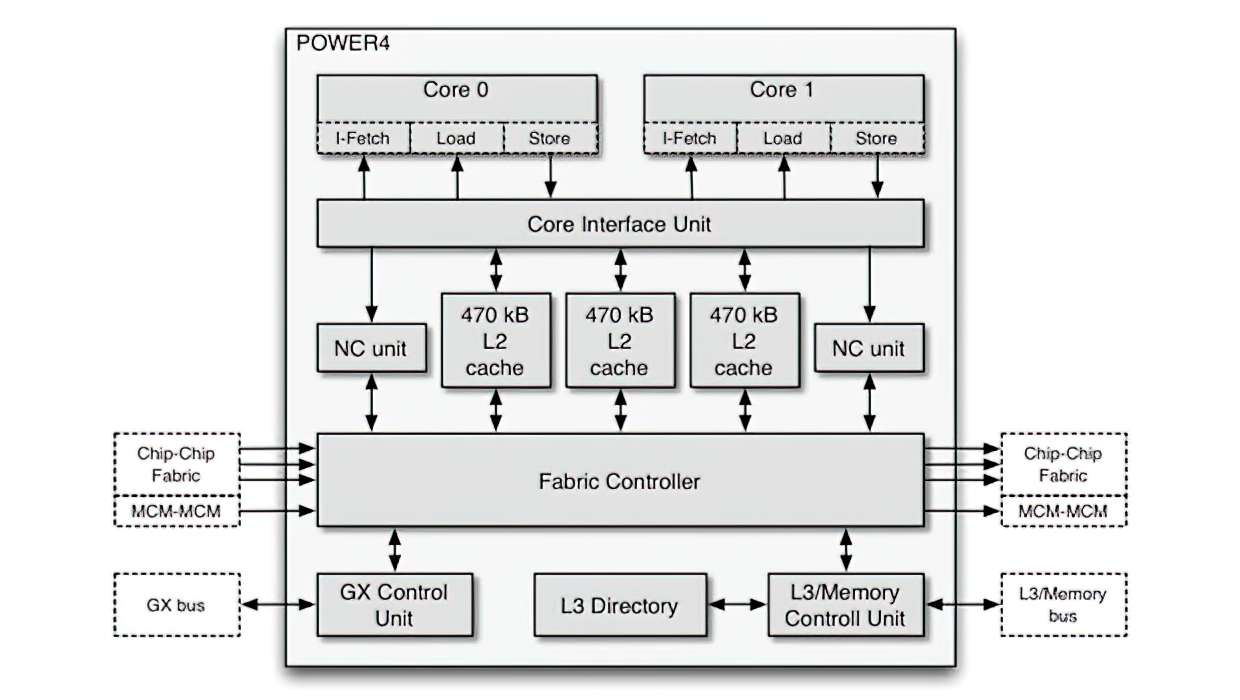
\includegraphics[width=\textwidth]{img/power4-2x.png}
	{\hspace*{\fill}\tiny\textit{Forrás: ibm.com}}	
\end{figure}
}

\uncover<3-> {
\begin{alertblock}{Folyamatok, szálak}
	\begin{itemize}
		\item Folyamat
		\begin{itemize}
			\item Egy futó program elnevezése
		\end{itemize}
		\item Szál
		\begin{itemize}
			\item Egy futó műveletsor elnevezése
			\item Egy folyamatot több szálra tudunk bontani
			\item Mindig \q{párhuzamosan} futnak
		\end{itemize}
	\end{itemize}
\end{alertblock}
}

\end{frame}